\section{Flow Models}
\subsection{Median Transformed CT}


We now fit statistical models for the response variable median TCT. Only data that were collected once the minnow trap was removed is included in this analysis. This corresponds to the six collection points in Figure 4.5. In general, as Log2(Flow) increases, we would expect `CT' to rise and hence `TCT' to decrease as the shed eDNA was washed out of the tank. We first fit a simple linear model, flow.l.one.line. This model only considers log2(Flow) as a predictor.



\begin{figure}[H]
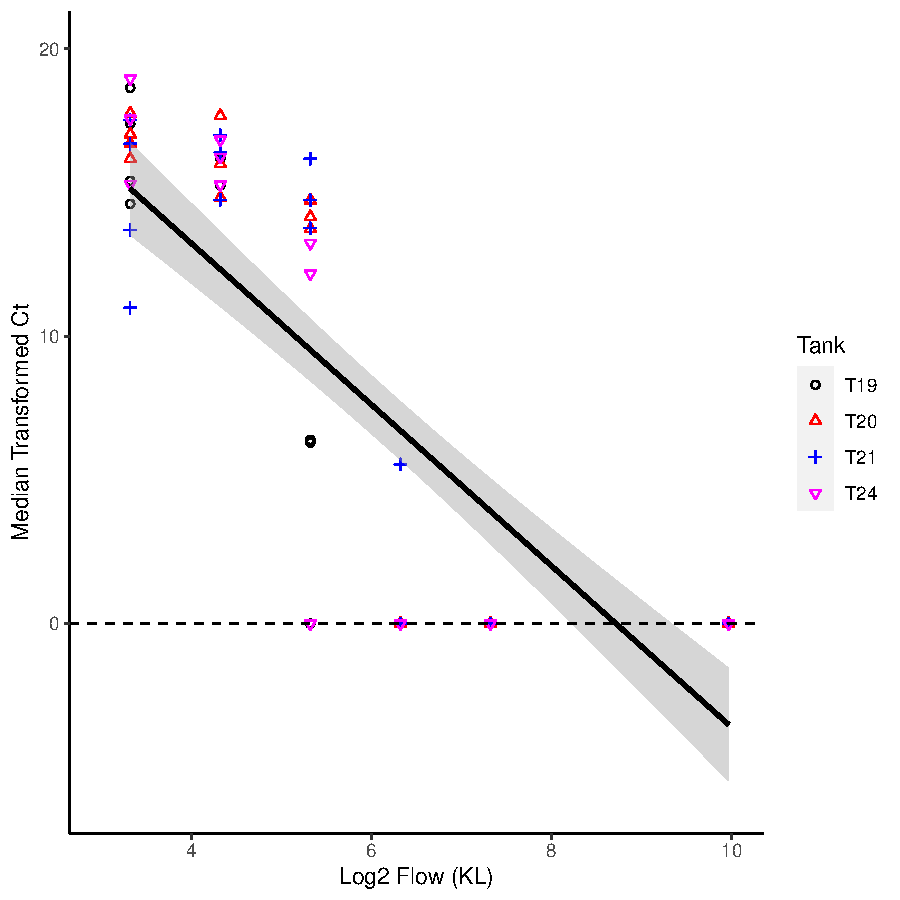
\includegraphics[scale=0.8]{Chapter4Images/flowmedtctgg.pdf}
\caption{Plot of Median TCT vs Log2(Flow) in kL, included is the simple linear model, flow.l.one.line and its associated 95\% confidence bands.}
\label{fig:flowmedtct}
\end{figure}


\begin{table}[H]

\includegraphics{Chapter4Images/flowloneline.pdf}
\caption{Parameter estimates and standard errors for a simple linear model on Median TCT. This model only considers log2(Flow) as a predictor. Model: flow.l.one.line. The $R^{2}$ for this model is 0.680.}
\label{fig:flow11}
\end{table}

Figure~\ref{fig:flowmedtct} is the plot of the regression line flow.l.one.line. Median Transformed CT is taken over each Sample.replicate vs Log2(Flow). Notice that at a certain point, median TCT approaches zero. That is, we no longer are detecting eDNA past a certain value of Log2(Flow). We later use alternative models that account for this fact as it does not make sense to predict negative median TCT values. Table~\ref{fig:flow11} provides the estimates of the model flow.l.one.line. The estimated intercept is 24.46 with a standard error of 1.46 and the estimate for the flow term is -2.81. Both estimates have extremely small p-values, indicating high significance of both the intercept and slope. The $R^{2}$ is 0.68 which means our model does a reasonable job at explaining variation in the data. The $Pr(> |t|)$  is the p-value for the test of a zero parameter value. Since both the intercept and Log2(Flow) have small p-values, they should be included in the model.
 


\newpage

We now proceed as in Chapter 3, whereby we consider the impact of tank and interactions on the TCT values.  We fit a model flow.l.tank, that considers dilution as before and also considers the tank as a factor. This model thus allows the intercept to change depending on the tank; however, the slope for each tank remains constant. 

\vspace{5mm}


\begin{table}[H]
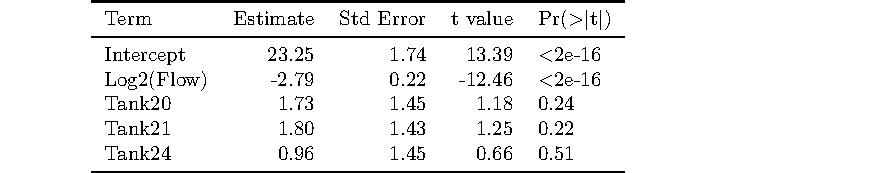
\includegraphics{Chapter4Images/flowltank.pdf}
\caption{Parameter estimates and standard errors for a linear model on Median TCT. This model allows for differing intercepts among tanks. Model: flow.l.tank.  The $R^{2}$ for this model is 0.689.}
\label{fig:flow12}
\end{table}

Table~\ref{fig:flow12} is a summary of our model that  includes the tank number as a factor.  As before, there is a high level of significance for the intercept and flow terms. Each tank has an associated coefficient term. The baseline tank is tank 19. For example, a sample corresponding to Tank 20 would have an intercept of 23.25+1.73 and a slope of -2.79. The individual p-values for each tank do not immediately appear significant. However, this does not guarantee that tank itself is not important. To conclude that, we would need to compare this model with a model that does not contain tanks, we can do this using `anova'.  The $R^{2}$ for flow.l.tank 0.689, which is only slightly larger than the $R^{2}$ for flow.l.one.line. Moreover, the adjusted $R^{2}$ which accounts for number of predictors is now actually less than the $R^{2}$ of flow.l.one.line.

\newpage

We also fit a  model flow.l.four.line that considers flow, tank as a factor and also the interaction between tank and biomass. This will allow not only for differing intercepts, but also differing slopes for each tank.

\vspace{5mm}

\begin{table}[H]
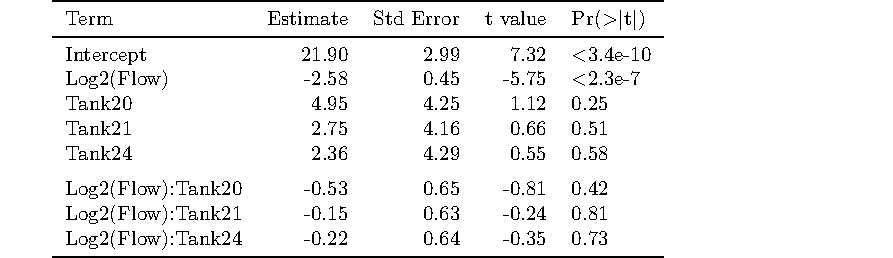
\includegraphics{Chapter4Images/lfourlinemed.pdf}
\caption{Parameter estimates and standard errors for a model that includes tank and the interaction between tank and Log2(Flow). Intercepts and slopes are allowed to differ for each tank. Model: flow.l.four.line. The $R^{2}$ for this model is 0.692.}
\label{fig:flow13}
\end{table}

Table~\ref{fig:flow13} summarizes the model flow.l.four.line. This model includes tank and the interaction between tank and Log2(Flow). The output indicates that neither tank, nor the interaction are significant. The interaction terms are multiplications of flow and the tank indicator terms. These terms would cause a different slope depending on which tank the sample was taken.

\newpage

 We now preform an `anova (extra sum of squares)' test to see which of our models is significant; 
\vspace{5mm}

\begin{table}[H]
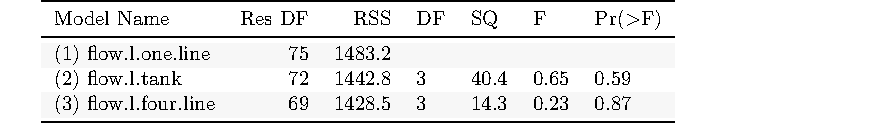
\includegraphics{Chapter4Images/anovamed.pdf}
\caption{Extra sum of squares test results for  the three flow models on median TCT.}
\label{fig:anovaflow}
\end{table}


  
  
Table~\ref{fig:anovaflow} provides the results of the extra sum of squares test. The full model,  flow.l.four.line allows both the intercept and slopes to differ depending on which tank the sample is taken from.
We compare this model with the model flow.l.tank to test for the hypothesis of differing slopes between tanks. Because the p-value is large (p=0.87) , we cannot reject the hypothesis that the coefficient for additional slopes is zero. Similarly, when comparing flow.l.tank with flow.l.one.line, the hypothesis is that the coefficient that determines differing intercepts among tanks is zero. Because the p-value is again large (p=0.586), we cannot reject (at the 0.05 significance level) the hypothesis that the coefficient is zero. Hence, we conclude that both tank and the interaction between tank and Log2(Flow) are not needed in our models.









